%!TEX root = main.tex

\chapter{Parametrised constraints}\label{chapter:parametrised:constraints}
This chapter covers the treatment of linear discrete time systems subject to additive 
disturbances in a robust model predictive control framework.
%
The disturbance affecting the system is considered belong to polyhedral sets, .i.e.
realisations satisfy a number of linear inequalities, furthermore the considered sets 
depend on parameters. 
%
Two different types of parametrisations are considered: 
%
\begin{enumerate}
\item State and input dependent sets,
\item uniformly scaled sets.
\end{enumerate}
%
The framework required to handle state and input dependent disturbance sets covers the 
treatment of scaled sets almost entirely and will hence be the main emphasis of this
chapter.
%
%
\section{Parametric convex sets}\label{sec:parametric:convex:sets}
In this section we discuss \emph{parametric convexity}, an attribute of sets valued maps 
(so called point-to-set maps, see e.g.~\cite{Hogan:1973}) we exploit later on to prove 
convexity of a generalised Pontryagin difference.
%
\begin{defn}[Parametric Convexity]\label{def:parametric:convexity}
	Let $X\subseteq\mathbb R^n, Y\subseteq\mathbb R^m$, let $\mathcal P(Y)$ denote the power set of $Y$, 
	and $T:X\rightarrow \mathcal P(Y)$, $X\ni s\mapsto T(s)\subset Y$ be a 
	continuous point-to-set map. The map $T$ is called \emph{parametrically convex} if it satisfies
	\begin{equation}\label{eq:def:parametrically:convex}
	T(\lambda s_1 + (1-\lambda)s_2)\subseteq\lambda T(s_1) \oplus (1-\lambda) T(s_2)
	\end{equation}
	for all $s_1,s_2\in X$ and $\lambda\in[0,1]$.
\end{defn}
%
For sets to be parametrically convex the dimensions~$n$ and~$m$ do not need to be the same, see e.g.
Figure~\ref{fig:parametrically:convex:set} for a piecewise affinely scaled square where~$n=1$ and $m=2$.
%
\begin{figure}
\centering
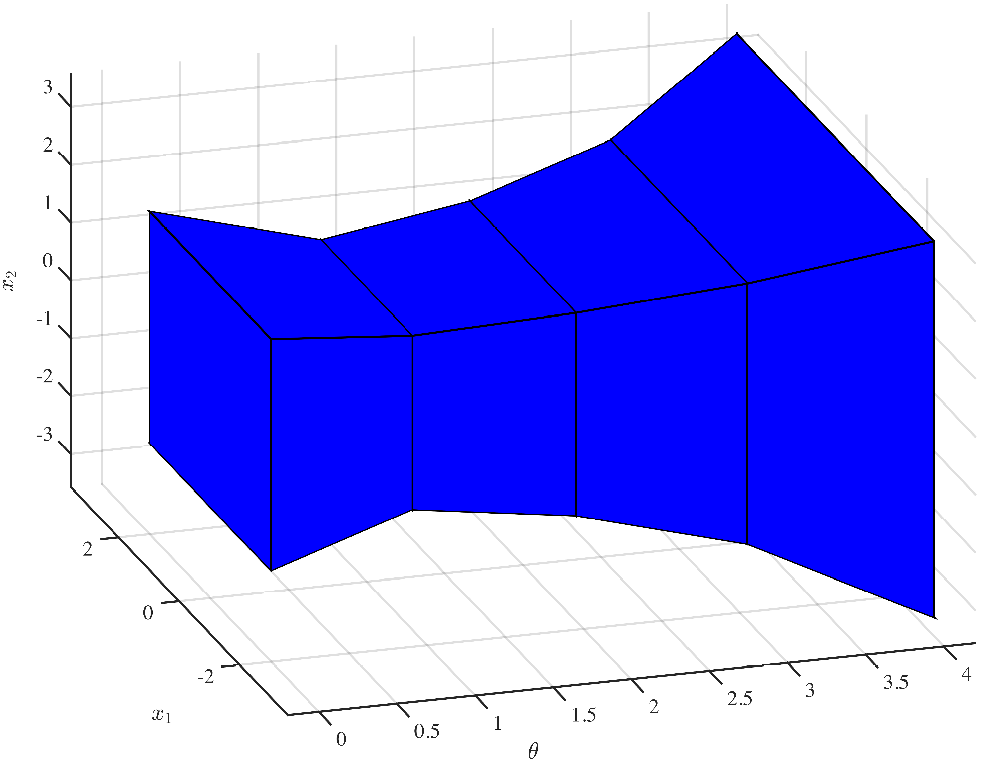
\includegraphics[width=.7\textwidth]{ParametricConvexSet}
\caption[A parametrically convex set.]{The piecewise affine parametric set $\mathcal X(\theta)$ 
defined by $\mathcal X(\theta)\mathrel{\mathop:}=\left\{x:\norm{x}_\infty\leq\max\{-\frac{1}{2}
\theta+2,\frac{1}{4}\theta+\frac{1}{5},\frac{1}{2}\theta+\frac{3}{4},\theta-\frac{3}{4}\}\right\}$ 
for $\theta\in[0,4]$. $\mathcal X(\theta)$ is parametrically convex in~$\theta$.}
\label{fig:parametrically:convex:set}
\end{figure}
%
Notice that Definition~\ref{def:parametric:convexity} does not require convexity of~$T(s)$ for all
$s\in X$, we will however only treat maps~$T$ for which $T(s)$ is convex.
%
In order to compute maximal positive invariant sets for the considered system we need to generalise
the Pontryagin set difference (see e.g.~\cite{blanchini:2007}) to accommodate parametrically convex sets.
%
\begin{defn}[Parametric Pontryagin Difference]\label{def:parametric:pontryagin:difference}
	Let $S\subseteq X$ and let $T:X\to\mathcal P(X)$ be a continuous point-to-set map such that
	$T(x)$ is convex for all $x\in X$, then the \emph{parametric Pontryagin difference} 
	$S\ominus T(S)$ is 
	\begin{equation}\label{eq:definition:parametric:pontryagin:difference}
		S\ominus T(S) = \left\{x\in X: \{x\} \oplus T(x)\subseteq S\right\},
	\end{equation}
	where $T(S)$ denotes the image of $S$ under the map $T$. 
\end{defn}
%
At first it may seem sensible to generalise the Pontryagin difference even further and define
%
\begin{equation}\label{eq:extended:parametric:pontryagin:difference}
\begin{split}
	S\ominus T(R) &= \{x:\{x\}\oplus T(r)\subseteq S\,\forall\, r\in R\}\\
	&=\{x:\{x\}\oplus\bigcup_{r\in R} T(r)\subseteq S\}.
\end{split}
\end{equation}
%
However, since $\bigcup_{r\in R} T(r)$ may or may not be convex, we can not make any useful
statements about $S\ominus T(R)$. 
%
In the case that~$T(x)$ is constant, i.e. $\bigcup_{x\in X}T(x)=T(x)=:C$,
we see that $S\ominus T(S)=S\ominus C$ which is the Pontryagin difference for regular sets.
%
For the parametric Pontryagin difference of a convex set and a parametrically convex map we 
have the following result.
%
\begin{thm}\label{thm:convexity:of:pontryagin:difference}
  Let $S\subseteq X$ be a convex set and let $T:X\rightarrow\mathcal P(X)$ be a parametrically convex point-to-set
  map such that $T(x)$ is convex for all $x\in X$, then $S\ominus T(S)$ is convex.
\end{thm}
%
\begin{proof}
To prove the convexity of $ Z :=  S\ominus T( S)$ we pick any $z_1,z_2\in Z$, then
by definition of the parametric Pontryagin difference, we have
%
\begin{equation}
	\{z_i\} \oplus T(z_i) \subseteq S,\; i=1,2.
\end{equation}
%
To see that $ Z$ is convex we show that line segments between
all possible $z_1$ and $z_2$ are subsets of $ Z$, i.e.~for all $\lambda \in [0,1]$,
\begin{equation}
\begin{aligned}
	\{ \lambda z_1 + (1-&\lambda)z_2
	\}\oplus T\left( \lambda z_1 + (1-\lambda)z_2\right)\\
	\subseteq&\left\{ \lambda z_1 + (1-\lambda)z_2
	\right\}\oplus \lambda T(z_1) \oplus (1-\lambda)
	T(z_2)\\
	\subseteq &\lambda\underbrace{(\{z_1\}\oplus T(z_1))}_{\subseteq S}\oplus
	(1-\lambda)\underbrace{(\{z_2\}\oplus T(z_2))}_{\subseteq S}\\
	\subseteq& Z
\end{aligned}
\end{equation}
%
where the last inclusion follows from the convexity of $\mathcal S$.
\end{proof}
%
Now consider a parametrically convex set of the form
%
\begin{equation}\label{eq:parametric:polyhedron}
	T(s)=\{t:Gt\leq H(s)\},
\end{equation}
%
where each row of $H(s)$ is a convex function in $s\in S$, i.e. each element $H_i(s)$ of 
$H(s)$ satisfies $H_i(\lambda s_1+(1-\lambda)s_2)\leq \lambda H_i(s_1)+(1-\lambda)H_i(s_2)$ 
for all $\lambda\in[0,1]$ and $s_1, s_2\in S$. 
%
We will use sets for which $H(s)$ is piecewise affine in $s\in S$, i.e. sets
for which $H_i(s) = \max_k\{f_k s + g_k\}$.
%
For sets of this type we have the following result.
%
\begin{thm}\label{thm:convex:parametric:set}
  The point-to-set map $T(s)$ defined by~\eqref{eq:parametric:polyhedron} is parametrically 
  convex for all $s\in S$ if $H(s)$ is elementwise convex in $s\in S\subseteq X \subset 
  \mathbb R^n$.
\end{thm}
%
\begin{proof}
To show that $T(\lambda s_1 + (1-\lambda)s_2)\subseteq \lambda T(s_1) \oplus(1-\lambda)
T(s_2)$ for all $\lambda \in [0,1]$ and $s_1, s_2\in S$ we note that
%
\begin{equation}
\begin{aligned}
  T&(\lambda s_1 + (1-\lambda)s_2)\\
  =& \{t:\; G t \leq H(\lambda s_1 + (1-\lambda)s_2)\}\\
  \subseteq& \{t:\;Gt\leq\lambda H(s_1)+(1-\lambda) H(s_2)\}\\
  =&\{t:\;Gt\leq\lambda H(s_1)\}\oplus\{t:\;Gt\leq(1-\lambda)H(s_2)\}\\
  =&\lambda T(s_1)\oplus(1-\lambda) T(s_2).
  \end{aligned}
\end{equation}
%
\end{proof} 
%
Notice that rays and vertices of $T(s)$ as defined in~\eqref{eq:parametric:polyhedron} will
be linear combinations of $H_i(s)$, this implies that for piecewise affine $H(s)$ rays
and vertices $t_k(s)$ will themselves be piecewise affine in $s\in S$, we will exploit
this fact later on.
%
%
%
%
%
\section{Example}\label{sec:example:linearisation:error:as:state:dependent:constraint}
In this section we derive a disturbance set that is of the form~\eqref{eq:parametric:polyhedron}
with a piecewise affine right hand side~$H(s)$. 
%
Consider a discrete time nonlinear system of the form
%
\begin{equation}
	x^+ = f(x,u)
\end{equation}
%
with $x_e=f(x_e,u_e)$ as an equilibrium point. 
%
Close to the equilibrium point the dynamics can be approximated by ${\tilde x}^+ = A \tilde x 
+ B\tilde u$ with $\tilde x = x-x_e$ and $\tilde u = u - u_e$ and the linearisation matrices
$A = \frac{\partial f}{\partial x}\vert_{(x_e,u_e)}$ and $B = \frac{\partial f}{\partial u}
\vert_{(x_e,u_e)}$.
%
We want to describe the dynamics of the nonlinear system with those of its linearisation considering
an additive disturbance. 
%
I.e. we want that for all $x\in X_c$ and $u\in U_c$ there exists a realisation 
$v\in V(x,u)$ such that the identity $f(x,u)=Ax + B u + v$ holds. 
%
In order to derive a parametrised set $V(x,u)$ such that the desired identity holds we use
the mean value theorem (see e.g.~\cite{Apostol:1974}):
%
\begin{thm}[Mean Value Theorem]\label{thm:mean:value:theorem}
Let $g : \mathcal X \rightarrow\mathbb R^m$ be continuously
differentiable, $\mathcal X\subset\mathbb R^n$ be open,
and $x \in\mathcal X$, $h \in\mathbb R^n$ be such that 
$x + th \in\mathcal X$ for all $t\in [0 ,1]$. Then
\begin{equation}
	g(x+h) = g(x) + \left(\int_0^1 \frac{\partial g}{\partial x}(x+th)dt\right)\cdot h.
\end{equation}
\end{thm}
%
We can use this to state
%
\begin{equation}
\begin{split}
	f(x_e+x,u_e+u)-A(x_e+x)-B(u_e+u) = \underbrace{f(x_e,u_e) - A x_e - B u_e}_{=0} \\
	+ \int_0^1\left(\frac{\partial f}{\partial x}(x_e+tx,u_e+tu) \cdot x + 
	\frac{\partial f}{\partial u}(x_e+tx,u_e+tu) \cdot u \right) dt -Ax-Bu\\
	= \underbrace{\left(\int_0^1 \frac{\partial f}{\partial x}(x_e+tx,u_e+tu) dt - A\right)}_{H^x} x + 
	\underbrace{\left(\int_0^1 \frac{\partial f}{\partial u}(x_e+tx,u_e+tu) - B \right)}_{H^u} u.
\end{split}
\end{equation}
%
This means that for any given $(x,u)\in X\times U$ we can compute an additive disturbance $v=H^x x + H^u u$
such that $f(x_e+x,u_e+u)-Ax-Bu = v$.
%
Assume we had all possible $H^x$ and $H^u$ for all $(x,u)\in X\times U$ given, clearly then 
$\min\{H^x x + H^u u\} \leq f(x_e+x,u_e+u)-Ax-Bu \leq \max\{H^x x + H^u u\}$ holds true.
%
For general nonlinear systems there is no way to obtain an analytic solution for $H^x$ and $H^u$,
so instead $K$ samples of $X\times U$ have to be used to obtain a description of 
the disturbance set
%
\begin{equation}\label{eq:derivation:of:PWA:disturbance:set}
\begin{split}
	V^K(x,u) &= \left\{v: \min_{k\leq K}\{H^x_k x + H^u_k u\} \leq v \leq \max_{k\leq K}\{H^x_k x + H^u_k u\} \right\}\\
	&= \left\{v: v \leq \max_{k\leq K}\{H^x_k x + H^u_k u\} \wedge -v \leq \max_{k\leq K}\{-H^x_k x - H^u_k u\} \right\}
\end{split}
\end{equation}
%
Notice that sampling the set $\gimel(x,u) = \left\{v : \min\{H^x x + H^u u\} \leq v \leq \max\{H^x x + H^u u\}\right\}$ 
leads to an inner approximation which is convexified by taking its convex hull.
%
The set $V^K(x,u)$ as defined in~\eqref{eq:derivation:of:PWA:disturbance:set} is of the
type~\eqref{eq:parametric:polyhedron} with a piecewise linear right hand side. We may
want to add a constant term to accommodate model uncertainties.
%
%
%
%
\section{Maximal Positive Robust Invariant Sets}\label{sec:parametrised:MRPI:set}
In this section we present a way to calculate maximal robust positive invariant sets for
linear discrete time systems under the influence of additive perturbation.
%
We assume the perturbation to be constrained in sets which are piecewise affine in
the state, i.e.
%
\begin{equation}\label{eq:definition:PWA:uncertainty}
v\in \mathcal V(x) = \left\{v: Gv\leq\max_k\{H_k^x x + h_k\}\right\}.
\end{equation}
%
The definition of the maximal robust positive invariant set in this scenario is given as
the largest set satisfying
%
\begin{equation}\label{eq:MRPI:state:dependent:disturbance}
	\mathcal X^\infty = \left\{x: \Psi x + v \in\mathcal X^\infty\,\forall\, v\in\mathcal V(x)\right\},
\end{equation}
%
largest in the sense that it includes all smaller ones.
%
The implicit definition of~\eqref{eq:MRPI:state:dependent:disturbance} suggests a recursive 
computation of $\mathcal X^\infty$.
%
We assume system dependent state constraints $\mathscr X\subseteq\mathbb R^n$ are given,
we furthermore assume that $\mathscr X$ is polyhedral and contained in a band.
%
\begin{defn}[Band Property]
We say that a set $X\subseteq\mathbb R^d$ possesses the band property if there exists a 
matrix~$\Gamma\in\mathbb R^{p\times d}$ such that $X\subseteq B = \{x:\Gamma x\leq {\bf{1}}\wedge
-\Gamma x\leq{\bf{1}}\}.$
\end{defn}
%
That is, we assume that $\mathscr X= \{x:\Lambda_i x \leq \lambda_i \forall\, i\leq m\}\subseteq\{x:\Gamma x\leq{\bf{1}}\wedge
-\Gamma x\leq{\bf{1}}\}=:\mathscr B$.
%
In the following we discuss how to apply the principle of the Kolmanovsky and Gilbert 
algorithm\footnote{The concept was first introduced for 
unperturbed systems in 1991 by Gilbert and Tan~\cite{Gilbert:1991}, therefore all its derivatives 
are also referred to as the \emph{Gilbert and Tan algorithms}.} 
presented in~\cite{Kolmanovsky:1995}.
%
The algorithm is a recursive iteration: Starting from $\mathscr X$ we 'cut off' all such stated 
for which the successor state would violate~\eqref{eq:MRPI:state:dependent:disturbance}, i.e.
in the $n^\text{th}$~iteration we introduce constraints which enforce that the trajectories
of all points in the set would remain in the set for $n$~time steps.
%
This means that in the first iteration we enforce that for all points in the iterate the 
successor state is contained in the initial set $x^+\in X_0 = \mathscr X$:
%
\begin{equation}\label{eq:PWA:disturbance:first:iterate}
\begin{split}
	X_1 &= \{x: \Psi x + v\in X_0 \forall v\in\mathcal V(x)\}\\
	&=\{x:\Lambda_i(\Psi x +v)\leq \lambda_i \forall\,i\leq m_0\}\\
	&=\left\{x:\Lambda_i\Psi x + 
	\underbrace{\left\{\begin{array}{rl}\max& \Lambda_i v\\ 
	\text{s.t.}& v\in\mathcal V(x)
	\end{array}\right\}}_{\gamma_{1,i}^\ast(x)} \leq \lambda_i \forall\,i\leq m_0\right\}
\end{split}
\end{equation}
This requires the solution $m_0$ multi-parametric linear programs\footnote{Multi-parametric 
linear programs have been introduced as optimisation problems
in the late 1958 by~\cite{Courtillot:1958}. Various ways to solve mpLPs have been proposed.}
(mpLPs) in order to obtain~$v_{1,i}^\ast(x)$.
%
However, the solution of multi-parametric linear programs will be given by vertices 
of the constraint set, i.e. $\gamma_{1,i}^\ast(x)=\Lambda_i v_{k^\ast}(x)$ where $v_{k^\ast}(x)$
is the optimising vertex.
%
Recall that since $\mathcal V(x)$ is piecewise affine in $x$ its vertices will also be piecewise 
affine in $x$, i.e. there exists a representation $v_k(x)=\max_{l\leq K_k}\{W_l^k x + w_l^k\}$.
%
Notice that we do not need to solve all mpLP in order to compute $X_1$, adding all available
$W_l,w_l$ produces the desired set without solving $m_0$ mpLP:
%
\begin{equation}\label{eq:derivation:of:row:reduction:instead:of:mpLP}
\begin{split}
	X_1 &= \{x: \Lambda_i\Psi x + \gamma_{1,i}^\ast(x)\leq\lambda_i \,\forall i\leq m_0 \}\\
	&= \left\{x: \Lambda_i\Psi x + \max_l\{\Lambda_i (W_l^{k^\ast} x + w_l^{k^\ast}) \} \leq \lambda_i\, 
	\forall i\leq m_0 \right\} \\
	&= \left\{x: (\Lambda_i\Psi + \Lambda_i W_l^{k^\ast}) x \leq \lambda_i-\Lambda_i w_l^{k^\ast}\,
	\forall i\leq m_0, l\leq K_k  \right\} \\
	&= \left\{x: (\Lambda_i\Psi + \Lambda_i W_l^k) x \leq \lambda_i - \Lambda_i w_l^k\,
	\forall i\leq m_0, l\leq K_k, k\leq \kappa \right\}.
\end{split}
\end{equation}
%
The equalities~\eqref{eq:derivation:of:row:reduction:instead:of:mpLP} hold since only the 
inequalities which define~$\gamma_{1,i}^\ast(x)$ will define the set~$X_1$, i.e. we avoid
solving mpLP by introducing redundant inequalities, instead of $m_0$ supporting hyperplanes
we describe the set by $m_1 = m_0\cdot \kappa\cdot \prod_{k\leq \kappa} K_k$ hyperplanes with
a large number of them being redundant, here~$\kappa$ denotes maximal the number of vertices 
of~$\mathcal V(x),\,x\in\mathscr X$.
%
This seems to be a poor trade off, however, we can use inequality reduction algorithms at any
point of the iteration and reduce the number of hyperplanes~$m_1$ in the representation of~$X_1$.

The next set iterate~$X_2$ is then defined by
%
\begin{equation}
	\begin{split}
	X_2 &= \left\{x: \Psi (\Psi x + v) + \tilde v\in X_0\,\forall v,\tilde v\in\mathcal V(x) \right\}\\
	&= \{x\in X_1 : \Psi x + v \in X_1\,\forall v\in\mathcal V(x)\}\\
	&= X_1 \cap \{x: \Psi x + v \in X_1\,\forall v\in\mathcal V(x)\},
	\end{split}
\end{equation}
%
so that successive set iterates can be defined recursively.
%
The general iterate is given by:
%
\begin{equation}\label{eq:general:MRPI:iteration}
	X_{k+1} = X_k \cap \{x:\Psi x + v\in X_k\, \forall v\in\mathcal V(x)\}
\end{equation}
%
It is obvious that by its definition $X_{k+1}\subseteq X_k$, once $X_k\subseteq X_{k+1}$ holds
the iteration~\eqref{eq:general:MRPI:iteration} terminates.
%
$X_k\subseteq X_{k+1}$ implies that all $x\in X_k$ also satisfy $x\in X_{k+1}$, however
$X_{k+1}$ is defined as points to which the successor state is contained in $X_k$, therefore
$X_{k+1} = \mathcal X^\infty$. 

In the remainder of this section we will prove that the described algorithm terminates 
in a finite number of iterations.
%
Notice that the set iterates defined by~\eqref{eq:general:MRPI:iteration} can be formally
be defined by
%
\begin{equation}
	X_{k+1} = X_k \cap \{x: \Lambda_i\Psi^k x + \sum_{l=1}^{k-1} \gamma_{l,i}^\ast(x)\leq\lambda_i\,
	\forall i\leq m_0\},
\end{equation}
%
where
%
\begin{equation}\begin{split}
	\gamma_{l,i}^\ast(x) &= \max_j \Lambda_i\Psi^{l-1} v_j(x) \\
	&= \begin{array}{rl} \max_v &\Lambda_i\Psi^{l-1} v\\
		\text{s.t.} & v\in\mathcal V(x)\end{array} \\
	&= \begin{array}{rl} \max_{\tilde v} &\Lambda_i \tilde v\\
		\text{s.t.} & \tilde v\in \Psi^{l-1}\mathcal V(x) \end{array}.
\end{split}\end{equation}
%
So that~\eqref{eq:general:MRPI:iteration} becomes
%
\begin{align}
	X_{k+1} &= X_k \cap \left( \Psi^{-k-1} X_0\, \underset{1\leq i\leq k}{\bigominus} 
	\Psi^{i-1}\mathcal V(X_k) \right)\nonumber \\
	&=\bigcap_{l\leq k+1}\left(\Psi^{-l} X_0 \underset{1\leq i\leq l-1}{\bigominus} 
	\Psi^{i}\mathcal V(X_{l-1}) \right). \label{eq:MRPI:recursion:closed:form}
\end{align}
%
The structure of~\eqref{eq:MRPI:recursion:closed:form} is of central importance for the proof
of finite determinability of~$\mathcal X^\infty$.
%
The first statement we can prove is the following:
%
\begin{thm}\label{thm:band:implies:compactness}
Let the system constraints be contained in a band~$\mathscr X\subseteq \mathscr B 
=\{x: \Gamma x\leq{\bf{1}}\wedge -\Gamma x\leq{\bf{1}}\}$, let $0\in\mathcal V(x)$ for all $x\in\mathscr X$ 
and let the pair $(\Psi,\Gamma)$ be observable, then there exists a natural number $N\leq n$ such 
that~$X_N$ is compact.
\end{thm}
%
\begin{proof}
First recall the fact that $\mathcal A\ominus \mathcal B\subseteq\mathcal A$ if $0\in\mathcal B$,
see e.g.~\cite{blanchini:2007}, this fact extends to the parametric Pontryagin difference.
%
Therefore we have
%
\begin{equation}
	X_k= \bigcap_{l\leq k}\left(\Psi^{-l} X_0 \underset{1\leq i\leq l-1}{\bigominus} 
	\Psi^{i}\mathcal V(X_{l-1}) \right) \subseteq \bigcap_{l\leq k} \Psi^{-l} X_0
	= \bigcap_{l\leq k} \Psi^{-l}\mathscr X \subseteq \bigcap_{l\leq k} \Psi^{-l} \mathscr B.
\end{equation}
%
Note that observability of $(\Psi,\Gamma)$ is equivalent to the observability matrix
\[
	\Omega_o = \left(\begin{array}{c}
	\Gamma \\ \Gamma \Psi \\ \vdots \\ \Gamma \Psi^{n-1}
	\end{array}\right)
\]
%
has full rank.
%
This is equivalent to the null space of $\Omega_o$ being trivial, i.e.~$\ker\Omega_o=\{0\}$,
which implies that~$\{x: \Omega_o x \leq {\bf{1}} \wedge -\Omega_o x \leq {\bf{1}}\}$ is bounded.
%
Note further that
\begin{equation}
	X_n \subseteq \bigcap_{k\leq n} \Psi^{-k}\mathscr B = \left\{x:\underset{k\leq n}{\bigwedge} 
	\pm \Gamma\Psi^{k}x\leq{\bf{1}} \right\} =\{x: \Omega_o x \leq {\bf{1}}\wedge -\Omega_o x\leq{\bf{1}} \}.
\end{equation}
%
Therefore we conclude that $X_n$ is contained in a compact set, hence is itself bounded.
%
The case that~$N<n$ is possible for matrices $\Gamma$ with $\text{rank}(\Gamma)>1$.
\end{proof}
%
We can use Lemma~\ref{thm:band:implies:compactness} to prove the following statement:
%
\begin{thm}[\footnote{
	The earliest proof of finite determinability of the proposed algorithm was published 
	in~\cite[Theorem 4.2]{Kolmanovsky:1995}, the assumptions made for Lemma~\ref{thm:band:implies:compactness}
	and~\ref{thm:finite:terminability:MRPI:algorithm} coincide for the case of constant disturbance sets.
	%
	The formulation chosen here is more explicit than the one stated in~\cite{Kolmanovsky:1995}, since
	all conditions are on data available before initialising the algorithm.
	}]
\label{thm:finite:terminability:MRPI:algorithm}
Let the assumptions for Lemma~\ref{thm:band:implies:compactness} hold, let furthermore
$x^+=\Psi x$ be asymptotically stable and let $\mathcal V(x)$ be bounded for all $x\in\mathscr X$, 
then iteration~\eqref{eq:general:MRPI:iteration} with $X_0=\mathscr X$ terminates in a finite 
number of number of steps.
\end{thm}
%
\begin{proof}
Using~\eqref{eq:general:MRPI:iteration} we can easily see that if for some $k>0$
the set iterate $X_k$ is empty that implies that $X_k=\mathcal X^\infty = \emptyset$,
in this trivial case we can easily see that the algorithm terminates after $k$ iterations.
%
For the remainder of this proof we assume that all set iterates are non-empty.

Let $\rho$ denote the spectral radius of $\Psi$, since $\Psi$ is asymptotically
stable we have $\rho<1$.
%
Let $r_1$ be the radius of the largest ball contained in $X_0$ i.e. $\mathcal E(r_1)\subseteq X_0$ 
and let $r_2$ be the radius of smallest ball containing $V(x)$ for all $x\in X_0$.
%
Recall that $X_k = \bigcap_{l\leq k} D_l$, where $D_k$ is defined by
%
\begin{equation}
	D_l = \underbrace{\Psi^{-l} X_0}_{\mathcal S_1} \ominus 
	\underbrace{\left(\bigoplus_{1\leq i\leq l-1} \Psi^{i}\mathcal V(X_{l-1})\right)}_{\mathcal S_2}
\end{equation}
%
We can easily lower bound $\mathcal S_1$ by using $r_1$: $\mathcal S_1 = \Psi^{-l} X_0 
\supseteq \Psi^{-l}\mathcal E(r_1) \supseteq \mathcal E(\rho^{-l} r_1)$.
%
Recall that $X_l\subseteq X_{l-1}$ and therefore $X_l\subseteq X_0$ for all $l\geq0$.
%
We use this fact to obtain the containment $\mathcal S_2 = \bigoplus_{1\leq i\leq l-1} 
\Psi^{i}\mathcal V(X_{l-1})\subseteq \bigoplus_{1\leq i\leq l-1} \Psi^{i}\mathcal V(X_0)\subseteq
\bigoplus_{1\leq i\leq l-1} \Psi^{i}\mathcal E(r_2)\subseteq\bigoplus_{1\leq i\leq l-1} \mathcal E(\rho^{i} r_2)\subseteq
\mathcal E(\sum_{1\leq i\leq l-1}\rho^i r_2)\subseteq \mathcal E(\frac{1}{1-\rho} r_2)$.
%
In summary we can state that~$D_l$ consists of the exponentially expanding set~$\mathcal S_1$
subtracted by the set~$\mathcal S_2$ which is bounded, therefore~$D_l$ itself expands exponentially,
that is $D_l\supseteq\mathcal E(\rho^{-l} r_1 - \frac{1}{1-\rho} r_2)$.
%
Due to Lemma~\ref{thm:band:implies:compactness} we know that for $N\leq n$ the set iterate~$X_N$ is
bounded, let $r_3$ denote the smallest ball that contains $X_N$.
%
We can conclude that for $l$ such that $X_N\subseteq\mathcal E(r_3)\subseteq\mathcal 
E(\rho^{-l} r_1 - \frac{1}{1-\rho} r_2)\subseteq D_l$ holds the set $D_l$ covers
$X_N$, i.e. intersections with $D_l$ will not change $X_l$.
%
We can therefore give an upper bound on the number of iterations necessary for the algorithm
to terminate, it is given by the smallest integer $M$ such that
\begin{equation}\label{bnd:first:lower:bound:on:iteration:count}
	M\geq \frac{1}{\log(\frac{1}{\rho})}\left(\log\left(r_3+\frac{1}{1-\rho}r_2\right)-\log r_1 \right)
\end{equation}
is satisfied.
\end{proof}
%
Notice that the constants used in~\eqref{bnd:first:lower:bound:on:iteration:count} are not
quite convenient to compute, we can however compute bounds on $r_1,\, r_2$ and $r_3$ using 
singular values.
%
For this let $\bar\sigma(\Gamma)$ and $\underline\sigma(\Gamma)$ denote the maximal and the minimal
singular value of~$\Gamma$ respectively.
%
We know that~$\bar\sigma(\Gamma)\norm{x}\geq\norm{\Gamma x}$ and therefore $\bar\sigma(\Gamma)\norm{x}
\leq \sqrt{n}\Rightarrow \norm{\Gamma x}\leq\norm{\bf{1}}=\sqrt{n}$, that $r_1=\frac{\bar\sigma(\Gamma)}{\sqrt{n}}$
follows form standard result for singular values, see e.g.~\cite{Golub:1996}.
%
We use a similar argument to obtain a bound on $r_3$ before deriving a bound on $r_2$:
%
It is easy to see that the radius of the largest ball containing $X_N$ is given by the maximal
norm of its vertices, i.e. $r_3=\max_{i}\norm{x_i}$ where $x_i$ satisfies $\Omega_{o,\mathscr{A}_i} x_i={\bf{1}}$
and $\Omega_{o,\bar{\mathscr A}_i}x_i<{\bf{1}}$.
%
From this we can deduce that
%
\begin{equation}\begin{split}
	\sqrt{n}=\norm{\bf{1}}=\norm{\Omega_{o,\mathscr{A}_i}x_i}\geq\underline\sigma(\Omega_{o,\mathscr{A}_i})\norm{x_i}
	=\underline\sigma(\Gamma_{\mathscr{A}_i}\cdot \text{diag}(I,\Psi,\dots,\Psi^{n-1}))\norm{x_i}\\
	\geq\underline\sigma(\Gamma_{\mathscr{A}_i})\underline\sigma( \text{diag}(I,\Psi,\dots,\Psi^{n-1}))\norm{x_i}
	\geq\underline\sigma(\Gamma_{\mathscr{A}_i})\underline\sigma(\Psi)^{n-1}\norm{x_i}\\
	\geq\underline\sigma(\Gamma)\underline\sigma(\Psi)^{n-1}\norm{x_i},
\end{split}\end{equation}
%
which implies that we can get the upper bound $r_3\leq\frac{\sqrt{n}}{\underline\sigma(\Gamma)
\underline\sigma(\Psi)^{n-1}}$.
%
In order to obtain an estimate on $r_2$ we follow a similar argumentation:
%
\begin{equation}\begin{split}
	\bar\sigma(H_{k^\ast})\norm{x}+\norm{h_{k^\ast}}=\max_k\{\bar\sigma(H_k)\norm{x}+\norm{h_k}\}\geq
	\norm{\max_k\{H_k x + h_k\}_{\mathscr{A}_i}}\\ 
	=\norm{G_{\mathscr{A}_i}v_i} \geq\underline\sigma(G_{\mathscr A_i})\norm{v_i}
	\geq\underline\sigma(G)\norm{v_i}.
\end{split}\end{equation}
%
Notice that with only the assumptions made in Lemma~\ref{thm:finite:terminability:MRPI:algorithm}
we have no way to bound~$\norm{x}$ in order to obtain an upper bound on~$r_2$,
however, if we assume that~$X_N$ is not empty we can use the bound on~$X_N$, i.e.~$r_3$.
%
This is reasonable since we are interested in the asymptotic behaviour of the set rather than
exact bounds on intermediate iterates, hence $r_2\leq\frac{\bar\sigma(H_{k^\ast})r_3+\norm{h_k}}
{\underline\sigma(G)}$ can be used as an estimate for the asymptotic behaviour of $\mathcal V(x)$
in the iteration.
%
All bounds and estimates on $r_1,\,r_2$ and $r_3$ can be calculated in advance to get an estimate
on how many iterations the described algorithm could require.
%
%
%
%
\section{Example}\label{sec:example:parametrised:MRPI:set}
\begin{figure}
\centering
\begin{lpic}{levitatingBall}
\lbl[tr]{25,3; $m g$}
\lbl[br]{25,25; $c\frac{i^2}{y^2}$}
\lbl[bl]{49,17; $y$}
\lbl[bl]{56,55; $i$}
\end{lpic}
\vspace{-2mm}
\caption{Levitating ball system.}
\label{fig:levitating:ball}
\end{figure}
%
%
%
%
In this section we discuss the calculation of the MRPI set for a linearised simplified model of the magnetic 
levitation system depict in figure~\ref{fig:levitating:ball}. 
%
The system dynamics for the ball are given by $m \ddot y = m g - c\frac{i^2}{y^2}$, where $m,g,c,i$ and $y$ 
denote the mass of the ball, the gravitational constant, a constant factor, the current and the distance 
between the coil and the centre of the ball respectively.
%
For illustration purposes we neglect inductive dynamics and use the current $u=i$ as an input and the position
$y$ and its first derivative $\dot y$ as the states, i.e. $x = (y,\dot y)^T$. 
%
We find that any equilibrium has $\dot{y}=0$ and $u=\sqrt{\frac{gm}{c}} y$ for any positive position $y>0$. 
%
We use the method described in example~\ref{sec:example:linearisation:error:as:state:dependent:constraint}
to obtain a linear system with piecewise affine disturbance modelling the nonlinearites. 
%
Linearising the nonlinear differential equation $\dot x = f(x,u)$ around an equilibrium point $(\hat x, \hat u)$ 
gives the approximate linear model 
%
\begin{equation}
	 \Delta\dot{x} = \underbrace{\left(\begin{array}{cc}
	0 & 1 \\ \frac{2c\hat u^2}{m\hat x_1^3} & 0
	\end{array}\right)}_{\frac{\partial f}{\partial x}(\hat x,\hat
      u)}\Delta x 
+ \underbrace{\left(\begin{array}{c}
	0 \\ - \frac{2c\hat u}{m\hat x_1^2}
	\end{array}\right)}_{\frac{\partial f}{\partial u}(\hat x,\hat
      u)}\Delta u
\end{equation}
%
where $\Delta u = u -\hat{u}$ and $\Delta x \approx x-\hat{x}$.
%
We derive the discrete time dynamics with sampling rate $T_s$ using the Euler formula $x^+=x+T_s f(x,u) =:\tilde f(x,u)$ 
giving
%
\[
\Delta x^+ = A \Delta x + B \Delta u , \quad
\Biggl\{\begin{aligned} A &= I+T_s\frac{\partial f}{\partial  x}(\hat
  x,\hat u) \\
B &= T_s \frac{\partial f}{\partial u}(\hat x,\hat u)
\end{aligned}
\]
%
Although this system has a control input, the algorithm for computing the MRPI set is applicable since we consider 
the closed loop system under linear feedback  $u=Kx$, where $K$ is designed to satisfy a robust Lyapunov condition 
described in Appendix~\ref{app:terminal:controller}, see e.g.~\cite{Boyd:94}.
%
We use the method derived in example~\ref{sec:example:linearisation:error:as:state:dependent:constraint} to 
obtain piecewise affine disturbance set, such that
%
\begin{equation}
	\tilde x^+ = (A+ BK)\tilde x + v,\quad v\in\mathcal V(\tilde x) = \left\{v:v\leq\max_{k} 
	\{(H_k^x + H_k^u K) \tilde x+ h_k\}
	\right\}
\end{equation}
%
covers the nonlinear system.
%
As numerical values we chose $T_s=30ms, C=1, m=100g, \hat x_1 = 50mm$ and sample
the sets $\mathcal X=\{x:\abs{x_1- \hat x_1}\leq 1mm\wedge \abs{x_2}\leq 105\frac{mm}{s}\}$, 
$\mathcal U=\{u:\abs{ u-\hat u}\leq10mA\}$ with a total of~25 samples.
%
The presented algorithm for the computation of maximal robust positive invariant sets 
terminates after 3 iterations and produces the set depict in figure~\ref{fig:MRPI:set:levitating:ball}.
%
\begin{figure}
\centering
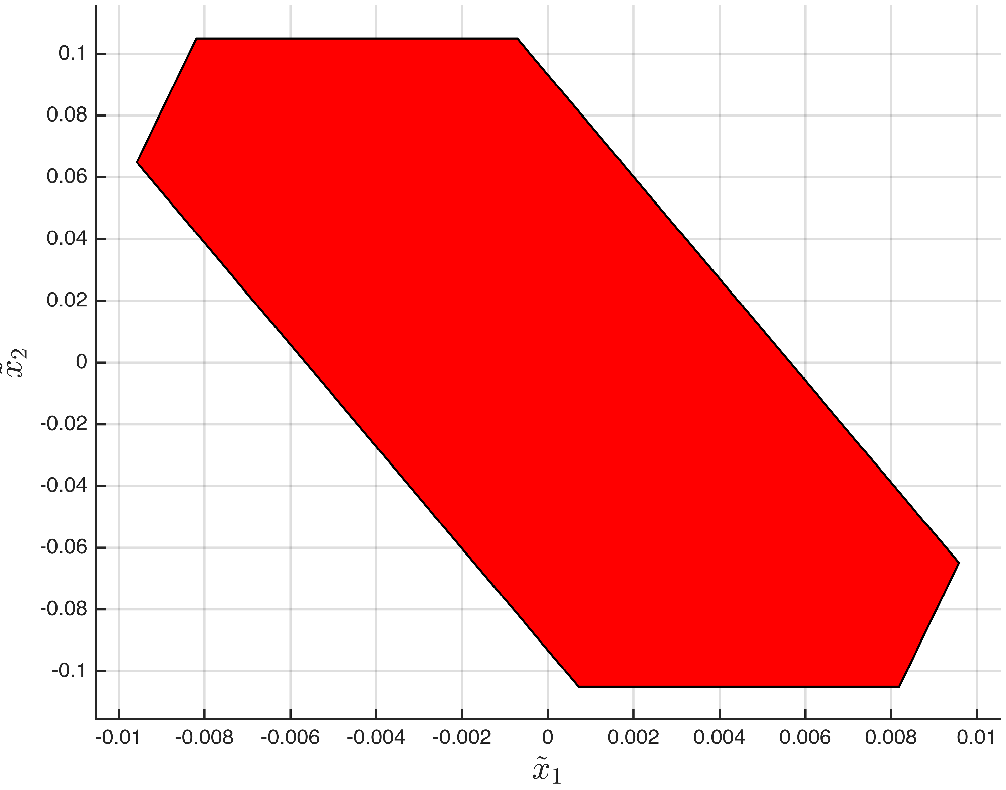
\includegraphics[scale=.65]{invariantSetStateDependant}
\caption{The maximal robust positively invariant set for the levitating ball system
has~6 supporting hyperplanes and the algorithm terminates after three iterations.}
\label{fig:MRPI:set:levitating:ball}
\end{figure}
%
%
%
%
%
\section{Problem Formulation}
In this section we present the min-max optimisation problem we will solve in order to
obtain a robust model predictive controller for a linear system subject to state and 
input dependent disturbance.
%
The cost functions we consider are quadratic, i.e.
%
\begin{subequations}\label{ch:par:con:the:problem}
\begin{equation}\label{ch:par:con:the:problem:cost}
	J_m^\ast(x) = \min_u \max_{w,x^+} \frac{1}{2}\left(x^T Q x + u^T R u - \gamma^2 w^T w\right) +
	J_{m-1}^\ast(x^+)
\end{equation}
%
subject to the system dynamics
%
\begin{equation}\label{ch:par:con:the:problem:system}
	x^+ = Ax + Bu + Dw,
\end{equation}
%
the disturbance constraints
%
\begin{equation}\label{ch:par:con:the:problem:disturbance}
	w\in\mathcal W(x,u) \mathrel{\mathop:}= \left\{w:Gw \leq \max_k\{H^x_k x + H^u_k u + h_k\}\right\}
\end{equation}
%
and the stage constraints
%
\begin{equation}\label{ch:par:con:the:problem:stage:constraints}
	(x,u)\in\mathcal Z_m =\left\{(x,u):\Xi_m^x x + \Xi_m^u u \leq \xi_m\right\}.
\end{equation}
\end{subequations}
%
Both the cost-to-go $J_{m-1}^\ast(x^+)$ in~\eqref{ch:par:con:the:problem:cost} as well as the
stage constraint set~$\mathcal Z_m$ in~\eqref{ch:par:con:the:problem:stage:constraints} are 
recursively defined.
%
The cost-to-go is initialised with $J_0^\ast(x) = \frac{1}{2}x^T P_0 x$ with~$P_0$ the unconstraint
optimal solution to the min-max problem, i.e.~$P_0=P$ in appendix~\ref{app:terminal:controller}.
%
The sets of stage constraints are computed in advance to satisfy the recursive definition
%
\begin{subequations}\label{ch:par:con:def:stage:constraints}
\begin{equation}
	\mathcal Z_m:=\left\{(x,u):Ax+Bu+Dw\in\mathcal X_{m-1} \forall w\in\mathcal W(x,u)\right\},
\end{equation}
%
where $\mathcal X_m$ denotes the projection of $\mathcal Z_m$, i.e. the constraints on the state alone
%
\begin{equation}
	\mathcal X_m\mathrel{\mathop:}=\left\{x:\exists u : (x,u)\in\mathcal Z_m\right\}.
\end{equation}
%
The state constraints $\mathcal X_m$ are initialised with the MRPI set~$\mathcal X^\infty$ 
of the system~\eqref{ch:par:con:the:problem:system} subject to the unconstrained optimal
feedback controller calculated in appendix~\ref{app:terminal:controller}, i.e.~
%
\begin{equation}
	\mathcal X_0 =\mathcal X^\infty \mathrel{\mathop:}= \{x: (A+BK)x+Dw\in\mathcal X^\infty\;
	\forall w\in\mathcal W(x,Kx)\},
\end{equation}
\end{subequations}
%
\par
%
In order to solve the min-max problem~\eqref{ch:par:con:the:problem} as a sequence of
multi-parametric quadratic programs, as presented in chapter~\ref{app:chp:mpqp}, we 
split~\eqref{ch:par:con:the:problem} into recursively defined maximisations and minimisations.
%
The maximisation is given by
%
\begin{subequations}\label{ch:par:con:the:maximisation}
	\begin{equation}
		\hat J_m^\ast(x,u) =\max_{w,x^+} -\frac{\gamma^2}{2} w^Tw + J_{m-1}^\ast(x^+)
	\end{equation}
	%
	subject to
	%
	\begin{equation}
		x^+ = Ax + Bu + Dw
	\end{equation}
	%
	and
	%
	\begin{equation}\label{ch:par:con:affine:rhs}
		Gw \leq \max_k\left\{H^x_k x + H^u_k u + h_k\right\}.
	\end{equation}
\end{subequations}
%
The minimisation is given by
%
\begin{subequations}\label{ch:par:con:the:minimisation}
	\begin{equation}
		J_m^\ast(x) = \min_u \frac{1}{2}\left( x^T Q x + u^T R u \right) + \hat J_m^\ast(x,u)
	\end{equation}
	subject to
	\begin{equation}
		\Xi_m^x x + \Xi_m^u u \leq \xi_m.
	\end{equation}
\end{subequations}
%
Now an active set solver as discussed in chapter~\ref{app:chp:mpqp} can be applied, with one additional
line search to determine the right hand side of~\eqref{ch:par:con:affine:rhs}.
%
This can be done as described in appendix~\ref{app:determining:pwa}.